% This is based on the LLNCS.DEM the demonstration file of
% the LaTeX macro package from Springer-Verlag
% for Lecture Notes in Computer Science,
% version 2.4 for LaTeX2e as of 16. April 2010
%
% See http://www.springer.com/computer/lncs/lncs+authors?SGWID=0-40209-0-0-0
% for the full guidelines.
%
\documentclass{llncs}

\usepackage{graphicx}

\begin{document}

\title{Skyscraper}
%
\titlerunning{Skyscraper}  % abbreviated title (for running head)
%                                     also used for the TOC unless
%                                     \toctitle is used
%
\author{André Cruz\inst{1} \and Edgar Carneiro\inst{2}}
%
\authorrunning{André Cruz \and Edgar Carneiro} % abbreviated author list (for running head)
%
%%%% list of authors for the TOC (use if author list has to be modified)
\tocauthor{André Cruz and Edgar Carneiro}
%
\institute{Faculdade de Engenharia da Universidade do Porto\\ Rua Roberto Frias, sn, 4200-465 Porto, Portugal,\\
\email{ feup@fe.up.pt},\\ WWW home page:
\texttt{http://www.fe.up.pt}}

\maketitle              % typeset the title of the contribution

\begin{abstract}
This article was written for the course unit ``Logic Programming'', from the course Master in Informatics and Computing Engineering.
This article purpose is to present how the program we developed is able to solve the decision problem that is the puzzle Skyscraper, independently of the booard size.
The program developed is also able to generate Skycraper puzzles as well. The program develop uses Logic Programming with Retrictions as the approach to solve and generate the puzzles.
\keywords{skycraper, PLR, sicstus, PLOG, FEUP}
\end{abstract}
%
\section{Introduction}
%
The main purpose of this project was to develop a program that would be able to solve either Decision Problems or Otimization Problems, by using Logic Programming with Restrictions.

Our group was assigned with a decision problem: the Skyscraper puzzle. Succintly, the puzzle consists of a grid that the player needs to fill, acordding to some given restrictions, and without repeting the same digits per column and per row.

The article approaches several thematics such as: what were the variables used and its domains, what were the constraints used and their implementation in the program, what is the labeling strategy implemented, what are the results of the developed program and what are the final conclusions obtained from developing the project and its pros.

%
\section{Problem Description}
%
Skyscraper consists of a puzzle where the player needs to fill a grid with digits from 1 to \textit{N} --- with \textit{N} being the the size of the grid --- where each row and column contains each digit exactly once. In the grid, each number represents the height of a building. The numbers outside the grid indicate how many buildings can be seen when looking from that direction. Taller buildings block the view of smaller buildiings, meaning that every number, when looking from that direction, beyond a number bigger than it, will not be taken into account.

The difficulty of the puzzle arises from the conjugation of two factors: the digits in rows and columns must all be distinct and the restrictions outside the grid.

\begin{figure}[h!]
\begin{center}
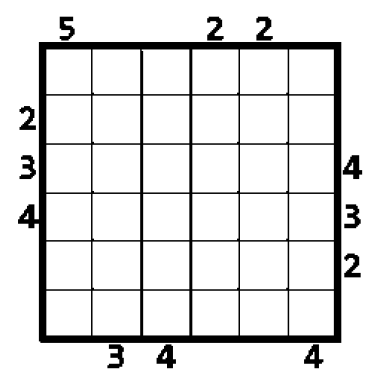
\includegraphics[height=6cm,width=6cm]{images/skyscraper_unsolved.png}
\caption{Unsolved 6x6 Skyscraper puzzle}
\label{Figure 1}
\end{center}
\end{figure}

\begin{figure}[h!]
\begin{center}
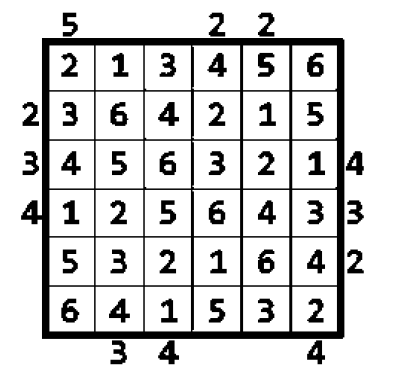
\includegraphics[height=6cm,width=6cm]{images/skyscraper_solved.png}
\caption{Solved 6x6 Skyscraper puzzle}
\label{Figure 2}
\end{center}
\end{figure}

%
\section{Approach}
%
\subsection{Decision Variables}
%
\subsection{Constraints}
%
\subsection{Evaluation Function}
%
\subsection{Search Strategy}
%
\section{Solution Presentation}
%
\section{Results}
%
\section{Conclusion and Future Work}
%


%
% ---- Bibliography ----
%
\begin{thebibliography}{5}
%
\bibitem {clar:eke}
Clarke, F., Ekeland, I.:
Nonlinear oscillations and
boundary-value problems for Hamiltonian systems.
Arch. Rat. Mech. Anal. 78, 315--333 (1982)

\bibitem {clar:eke:2}
Clarke, F., Ekeland, I.:
Solutions p\'{e}riodiques, du
p\'{e}riode donn\'{e}e, des \'{e}quations hamiltoniennes.
Note CRAS Paris 287, 1013--1015 (1978)

\bibitem {mich:tar}
Michalek, R., Tarantello, G.:
Subharmonic solutions with prescribed minimal
period for nonautonomous Hamiltonian systems.
J. Diff. Eq. 72, 28--55 (1988)

\bibitem {tar}
Tarantello, G.:
Subharmonic solutions for Hamiltonian
systems via a $\bbbz_{p}$ pseudoindex theory.
Annali di Matematica Pura (to appear)

\bibitem {rab}
Rabinowitz, P.:
On subharmonic solutions of a Hamiltonian system.
Comm. Pure Appl. Math. 33, 609--633 (1980)

\end{thebibliography}

\end{document}
